\chapter[Implementazione]{Implementazione}
Il software si pone l'obiettivo di verificare se una query e l'utilizzo del suo risultato sia corretto o meno. Per le query si tratta di verificare se sia abitata o meno. \textbf{mettere parte su utilizzo risultato ANDREA} Esso è formato da due componenti: un modulo Reasoner, scritto in Java che utlizza il reasoner HermiT\cite{HermiT} per stabilire l'abitabilità delle query, e un modulo scritto in OCaml che si occupa di parsare il programma  da un file testuale, genereare gli assiomi di Leinberger\ref{fig:LeinbergerAxiom} e richiamare il modulo Reasoner per le query. 
    
    \section{-Reasoner}
        Il modulo -Reasoner utilizza due risorse: 
            \begin{enumerate}
                \item Il file HermiT.jar \cite{HermiT}, che implementa il reasoner sviluppato dall'università di Oxford, capace di eseguire ragionamenti sulle ontologie.
                \item Il file DLQueryExample \cite{DLQueryExample} utilizzato per parsare una stringa in una ClassExpression, che è utilizzabile HermiT. 
            \end{enumerate}

        Ma come funziona il modulo? Esso prende in input, in formato stringa, una lista di assiomi di Leinberger, ognuno forma \(A_{x} : C\), con semantica \( A_{x}\sqsubseteq C \). 
        \\\(A_{x}\) è un concetto atomico. "C" è scritto nella "Manchester OWL syntax"\cite{ManchesterOWLSyntax}, e viene trasformato dal DLQueryParser in una ClassExpression. 

        Utilizzando poi la OWLDataFactory (factory delle OWLApi che permette la costruzione di OWLAxiom e di dichiarare OWLClass) e HermiT\cite{HermiT}, dichiariamo all'interno dell'ontologia tutti i concetti atomici, corrispondenti alle variabili della query, che compaiono negli assiomi di Leinberger. 

        \begin{figure}
            \centering
            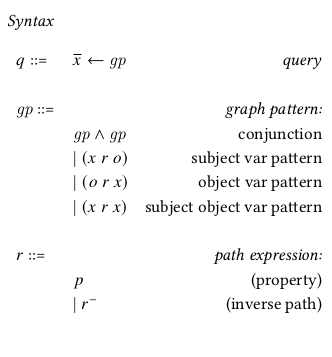
\includegraphics[width=\textwidth]{pictures/leinbergSyntax.png}
            \caption{sintassi delle query SPARQL CQ}
            \label{fig:declarationCode}
        \end{figure}
                
        Successivamente per ogni assioma creiamo un OWLSubClassOfAxiom, in cui viene specificata ogni concetto atomico come SubClass della sua ClassExpression corrispondente. 

        Infine chiediamo al reasoner HermiT di testare la soddisfacibilità di ogni concetto atomico presente negli assiomi di Leinberger. Se sono tutte soddisfacibili, allora significa che la query è abitabile, altrimenti non lo è.

        \section{-OCaml Module}
        L'idea alla base del modulo OCaml è la seguente: 
            \begin{enumerate}
                \item l'utente inserisce la query di cui testare l'abitabilità in un file di testo. 
                \item la query viene parsata in un tipo Query
                \item sul tipo Query vengono inferiti gli assiomi di Leinberger
                \item viene invocato il -Reasoner e gli vengono passati gli assiomi appena inferiti.
                \item il risultato viene mostrato all'utente
            \end{enumerate}

        Per generare il parser, ho utilizzato il programma OCamlyacc, un compilatore di compilatori, ispirandomi alla grammatica delle query descritta da Leinberger. %pagina 19

        Per definire i token che compongono la grammatica invece mi sono avvalso di OCamllex, un generatore di lexer. 

        Dunque, come funziona il Parser? Esso riconosce la grammatica e genera un tipo Query, che racchiude tutte le informazioni presenti allinterno della query in formato testuale. 

        Per esempio, scrivendo questa query sul file di input: 
        
        $$ query \ x \ <- \ (x \ type \ Pizza \ AND \ x \ hasTopping \ y \ AND \ y \ type \ GorgonzolaTopping) $$
        
        otteniamo il seguente tipo Query così costruito: %mettere?

        $$ Q \  (V \ x, \\
            CP(SP(V \ x,\ TYPE, \ ,\ CP)$$

        Successivamente, il tipo Query viene convertito in una lista di Axiom dalla funzione axiomiserQuery, che implementa le regole di derivazione di Leinberger\ref{fig:axiom}

        %%\begin{figure}
        %%    \centering
        %%    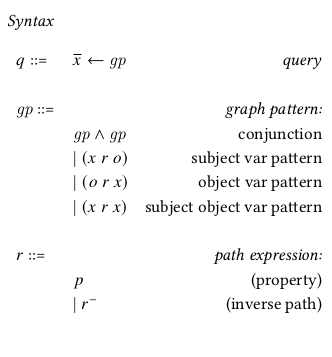
\includegraphics[width=\textwidth]{pictures/leinbergSyntax.png}
        %%    \caption{Sintassi delle query accettata}
        %%    \label{fig:LeinbergerSyntax}
        %%\end{figure}

        %%\begin{figure}
        %%    \centering
        %%    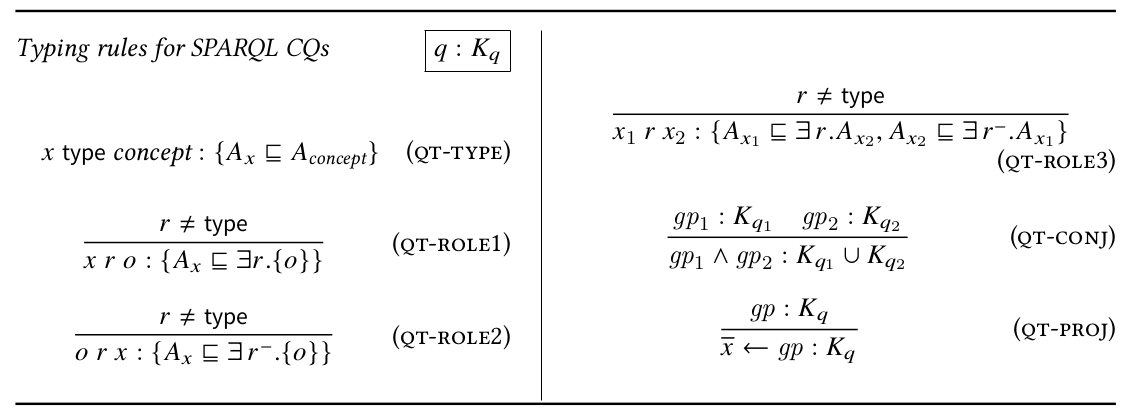
\includegraphics[width=\textwidth]{pictures/leinbergAxiom.png}
        %%    \caption{Regole di derivazione di Leinberger}
        %%    \label{fig:LeinbergerAxiom}
        %%\end{figure}

        

        
        Infine, la lista viene convertita in stringa secondo la sintassi \(A_{x} : C\). Viene dunque invocato il -Reasoner e gli viene passato come parametro la lista in formato stringa. La risposta, true o false, viene poi mostrata a video all'utente. 
    
    \section{Type Checking}
        \textbf{migliorare l'introduzione aggiungendo i datatype utilizzati}
        \\\\
        Il type checking del $\boldsymbol{\lambda_{DL}}$ proposto da Leinberger è basato su un semplice $\boldsymbol{\lambda}$\textbf{-calcolo tipato} con \textbf{Record} e \textbf{Liste}, insieme a nuove regole per tipare i nuovi construtti introdotti.
        In particolare è necessario assegnare dei tipi a:
        \begin{itemize}
            \item Query SPAQRL CQ
            \item Nodi dei grafi RDF ottenuti dalla esecuzione delle query 
        \end{itemize}
        Il primo caso è spiegato nelle sezioni precedenti. mentre il secondo richide l'aggiunta di un nuovo construttore di tipo. Siccome la logica descrittiva si pone
        l'obiettivo di dare struttura a una knowledge base, le \textbf{concept expressions} sono una scelta adeguata, in particolare è necessario controllare che i tipi dati alle query, ai nodi e alle proiezioni rispettino i vicoli imposti dagli assiomi 
        della ontologia di riferimento. Per questo motivo durante il type checking è necessario andare ad interrogare la knowledge base.
        \\Nelle successive sezioni commenteremo più nel dettaglio ogni regola rilevante del type system del linguaggio, mostrando una possibile implementazione in OCaml.

        \begin{figure}[h]
        \[\begin{array}{c}
            \myruleN{\Gamma,K \vdash t_1 : C_1 \quad K \vDash C_1 \sqsubseteq \exists r . \top}
            {\Gamma,K \vdash t_1.r : \textrm{List}(\exists r^- . C_1)}
            {T-PROJ}
            \qquad
            \myruleN{\Gamma,K \vdash : C \quad \Gamma,K \vdash t_2 : D}
            {\Gamma, K \vdash t_1 = t_2 : \textrm{Bool}}
            {T-EQ-NOM}
            \qquad
            \\\\
            \myruleN{\Gamma,K \vdash t_1 : \Pi_1 \quad \Gamma,K \vdash t_2 : \Pi_1}
            {\Gamma,K \vdash t_1 = t_2 : \textrm{Bool}}
            {T-EQ-PRIM}
            \qquad
            \myruleN{}{\Gamma,K \vdash o : \{o\}}{T-NOMINAL}
            \\\\
            \myruleN{q:K_q \quad \textrm{head}(q) = \{l_i^{i \in 1...m}\} \quad \forall x \in \textrm{Vars}(q) : K \cup K_q \nvDash A_x \sqsubseteq \bot}
            {\Gamma,K \cup K_q \vdash \textrm{query} \; q : \{l_i : A_{l_i}^{i \in 1...m}\} list}
            {T-QUERY}
            \\\\
            \myruleN{\Gamma,K \cup \{A_i \sqsubseteq C_i^{i \in 1...n}\} \vdash t : A_j^{1 \leq j \leq n} \quad K \cup \{A_i \sqsubseteq C_i^{i \in 1...n}\} \vDash A_j \sqsubseteq D^{1 \leq \leq n}}
            {\Gamma,K \vdash t : D}
            {T-ADD}
            \\\\
            \myruleN{K \vDash C \sqsubseteq D}{k \vdash C <: D}{S-CONCEPT}
        \end{array}\]
        \caption{nuove regole di tipo per $\lambda_{DL}$}
        \end{figure}
        \subsection{T-PROJ}
            La regola \textbf{T-PROJ} è usata per derivare il tipo di un nodo ottenuto attraverso la role projection.
            \\
            \[
                \myruleN{\Gamma,K \vdash t_1 : C_1 \quad K \vDash C_1 \sqsubseteq \exists r . \top}
                {\Gamma,K \vdash t_1.r : \textrm{List}(\exists r^- . C_1)}
                {T-PROJ}
            \]
            \\
            La prima ipotesi 
            $$\Gamma,K \vdash t_1 : C_1$$
            ci dice che con rispetto al contesto $\Gamma$ e alla knowledge base $K$ il termine $t_1$ a tipo $C_1$. Dove $C_1$ è una concept expression in logica descrittiva.
            $$K \vDash C_1 \sqsubseteq \exists r . \top$$
            la seconda invece afferma che la concept expression $C_1$ è un subconcept di $\exists r. \top$, ovvero che $C_1$ ha almeno un seccessore attraverso il ruolo $r$.
            $$ \Gamma,K \vdash t_1.r : \textrm{List}(\exists r^- . C_1) $$
            Dalle due ipotesi si può quindi concludere che il termine $t_1.r$ è una lista di nodi del grafo RDF, dai cui attraversando il ruolo $r^-$ si arriva a $C_1$, dove $r^-$ è ($\boldsymbol{\exists r^-.C_1}$).
            \\\\
            L'implementazione della regola T-PROJ è mostrata nella figura 4.3. la riga col commento \textbf{$\boldsymbol{\#}$1} corrisponde alla prima ipotesi della regola di derivazione,
            grazie al pattern matching dividiamo in due casi: il caso in cui il tipo è una concept expression (TyConcept(C) $\rightarrow$ ...) e qualsiasi altro caso ( \_ $\rightarrow$ ...).
             
            \begin{figure}[h] 
                \begin{minted}[escapeinside=||,mathescape=true, frame=lines, framesep=4mm, autogobble]{ocaml}
                    let rec typeof ctx t =
                        match t with
                        |$\vdots $|
                        TmRoleProj(fi, t, Property(s)) ->
                            (match t with                                
                            TyConcept(C) as t ->                                        #1
                                if subconcept C Exist(Property(s), Top) then            #2
                                    TyList(TyConcept(Exist(PropertyInverse(s), c)))     #3
                                else error fi "argument of role projection 
                                                is not a proper subconcept")
                            _ -> error fi "argument of role projection 
                                            is not a Concept Expression"
                        |$\vdots$|
                \end{minted}
            \caption{implementazione OCaml della regola T-Proj}
            \end{figure}
            Il commento \textbf{$\boldsymbol{\#}$2} indica la seconda ipotesi, la funzione \textbf{"subconcept C Exist(Property(s), Top)"} interroga la knowledge base controllando $C \sqsubseteq \exists r . \top$ e ritornando il risultato come
            booleano.
            Infine alla riga \textbf{$\boldsymbol{\#}$3} la funzione ritorna la lista di concept expression  $\exists r^- . C_1$.


        
        